% !TeX root = RJwrapper.tex
\title{Containers and R: the Rockerverse and beyond}
\author{by Daniel Nüst, Carl Boettiger, Robrecht Cannoodt, Dirk Eddelbuettel, Mark Edmondson, Colin Fay, Ben Marwick, Karthik Ram, Noam Ross, Nan Xiao, Lori Shepherd, Nitesh Turaga}

\maketitle

\abstract{%
The Rocker project provides widely-used Docker images for R across
different application scenarios. This articles surveys describe
downstream projects building upon Rocker. We also look beyond Rocker to
other projects connecting containerisation with R. These use cases and
the diversity of applications demonstrate the power of Rocker and
containerisation for collaboration, effectivity, scalability, and
transparency.
}


\hypertarget{introduction}{%
\section{Introduction}\label{introduction}}

The R community keeps growing: the number of new packages on CRAN keeps
on rising, meetups, conferences, online courses and unconferences
prosper, and the uptake in education and industry increases {[}REFs{]}.
All this cements the role of R as the lingua franca of statistics, data
visualisation, and computational research. Coinciding with the rise of R
was the advent of Docker {[}CITATION?{]} as a general tool for
development, distribution, and deployment of software. Combining both
these topics, the \emph{Rocker
Project}(\url{https://www.rocker-project.org/}) was introduced in 2014
and provides a number of
\href{https://en.wikipedia.org/wiki/Docker_(software)}{Docker} images
for various use cases as described in \citet{RJ-2017-065}. The
considerable uptake and continued evolution of the \emph{Rocker} suite
of containers has lead to numerous projects extending or building upon
\emph{Rocker} images ranging from reproducible research to production
deployments. This article presents this \emph{Rockerverse} of projects.
It also introduces related activities connecting the R language and
environment with other containerisation solutions. The main
contributions is a coherent picture of the current lay of the land of
containers in, with, and for \texttt{R}. This diversity includes
demonstrators, early prototypes, and mature projects.

\hypertarget{containerization-and-rocker}{%
\section{Containerization and
Rocker}\label{containerization-and-rocker}}

Docker, an application and service provide by the eponymous company, has
in just a few short years risen to prominence for development, testing,
deployment and distribution of computer software. While there are
related approaches such as LXC or Singularity, Docker has become
synomymous with ``containerization''---the method of taking software
artefacts and bundling them in such a way that use becomes standardized
and portable across operationg systems. In doing so, Docker had
recognised and validated the importance of one very important thread
that had been emerging, namely virtualization. By allowing multiple
concurrent applications or services to run concurrently on one host
machine without any fear of interference between them, an important
scalability feature had been realized. But Docker improved on
virtualization by accessing the host system---generally Linux---through
a much thinner and smaller shim than a full operating system emulation
or virtualization. This makes for more efficient use of system resources
and allowed another order of magnitude in terms of scalability of
deployment. {[}Reference?{]} While Docker makes use of Linux kernel
features, its importance was large enough so that some required aspects
of running Docker have been added to other operating systems to support
Docker there more efficiently too. {[}Win10; reference?{]}

The key accomplishment of Docker is to make a ``bundled'' aggregation of
software available to any system running Docker, without requiring much
else from the host. This is a rather attractive, and novel, proposition
which has lead to widespread adoption and use of Docker in a variety of
domains. It provided also a natural match for ``cloud deployment'' which
runs (or at least appears to run) ``seamlessly'' without much explicit
reference to the underlying machine, architecture or operating system.
Using containers on cloud hosted servers is a natural fit also because
these containers can be deployed with very littler in terms of
dependencies on the host system.

For statistical computing and analysis centered around R, the Rocker
Project has provided a variety of Docker containers since its start in
2014 \citep{RJ-2017-065}. The Rocker Project provides several lines of
containeres spanning to from building blocks with R-release or R-devel
to containers with RStudio Server and Shiny Server. Also of note is a
series of ``versioned'' containers which match the R release they
contain with the \emph{then-current} set of packages via the MRAN
Snapshot views of CRAN. {[}Maybe at a later point add forward reference
to other topics building on Rocker described here.{]}

\hypertarget{container-images}{%
\section{Container Images}\label{container-images}}

\hypertarget{images-for-alternative-r-distributions}{%
\subsection{Images for alternative R
distributions}\label{images-for-alternative-r-distributions}}

As outlined above, R is a widely-used language with a large community.
The large number of extension packages provides access to an unrivaled
variety of established and upcoming features. Nevertheless, special use
cases and experimental projects exist to test approaches or provide
features different to what \emph{``base R''} provides. These projects
stem both form academia and industry. \emph{Base R}, sometimes called
\texttt{GNU-R}, is the R distribution maintained by the
\href{https://www.r-project.org/contributors.html}{R Core Team} and and
provided via \href{https://cran.r-project.org/}{CRAN}.

\emph{Microsoft R Open}
(\href{https://github.com/nuest/mro-docker}{MRO}) is an R distribution
formerly known as Revolution R Open (RRO) before Revolution Analytics
was acquired by Microsoft. MRO is compatible with main R and it's
packages.sss ``It includes additional capabilities for improved
performance, reproducibility, and platform support.''
\citep{microsoft_mro} Most notably these capabilities are the MRAN
repository a.k.a. CRAN Time Machine, which is enabled by default, and
the (optional) integration with
\href{https://software.intel.com/en-us/mkl}{Intel® Math Kernel Library}
(MKL) for multi-threading in linear algebra operations
\citep{microsoft_multithread}. MRO does not provide official Docker
images, but a set of community-maintained \texttt{Dockerfile}s and
Docker images \texttt{nuest/mro} are available on Docker Hub at
\url{https://github.com/nuest/mro-docker} and on GitHub at
\url{https://github.com/nuest/mro-docker} respectively. The images are
inspired by the Rocker images and can be used much in the same fashion,
effectively a drop-in replacement allowing users to quickly evaluate if
the benefits of MRO + Intel® MKL apply to their use case. Version-tagged
images are provided for the latest bugfix release of recent R versions.
Extended license information about MKL is printed at every startup.

\emph{Renjin} is an interpreter for the R language running on top of the
\href{https://en.wikipedia.org/wiki/Java_virtual_machine}{Java Virtual
Machine} (JVM) providing full two-way access between Java and R code
\citep{wikipedia_renjin_2018}. It was developed to combine the benefits
of R, such scripting and extension packages, with the JVM's advantages
in the areas of security, cross-platform availability, and established
position in enterprise settings. R extension packages need to be
specially compiled and are distributed via the Java package manager
\href{https://en.wikipedia.org/wiki/Apache_Maven}{Apache Maven}, cf.
\url{http://packages.renjin.org/packages} for available packages.
Packages are loaded on demand, i.e.~at the first call to
\texttt{library()}. Not all R packages, especially one linking to binary
libraries, are available, e.g. \texttt{rgdal}
\footnote{\href{http://packages.renjin.org/package/org.renjin.cran/rgdal/1.4-4/build/1}{http://packages.renjin.org/package/org.renjin.cran/rgdal/1.4-4/build/1}}.

There are no offical Docker images for Renjin, but community-maintained
images for selected releases only are available under
\texttt{nuest/renjin} on Docker Hub and GitHub at
\url{https://hub.docker.com/r/nuest/renjin} and
\url{https://github.com/nuest/renjin-docker} respectively. These images
expose the command line interface of Renjin in a similar fashion as
Rocker images and allow an easy evaluation of Renjin's suitability, but
are not intended for production use.

\href{http://www.pqr-project.org/}{\emph{pqR}} is a ``a pretty quick
version of R''. \emph{pqR} fixes some opinionated issues in the R
language and is the basis for experimental features, e.g.~automatic
diffentiation\footnote{ \href{https://riotworkshop.github.io/abstracts/riot-2019-pqr.txt}{https://riotworkshop.github.io/abstracts/riot-2019-pqr.txt}}.
The source code development
\href{https://github.com/radfordneal/pqR/}{on GitHub} is a one man
project and it does not provide any Docker images. But especially
disruptive approaches may contribute to the development of the R
ecosystem, so the \texttt{nuest/pqr} images on Docker Hub and GitHub at
\url{https://hub.docker.com/r/nuest/pqr/} and
\url{https://github.com/nuest/pqr-docker} respectively.

\emph{FastR} is ``A high-performance implementation of the R programming
language, built on GraalVM'' (\url{https://github.com/oracle/fastr}). It
is developed by Oracle, connects R to the GraalVM ecosystem
\citep{wikipedia_graalvm_2019}, and also claims superior performance but
also targets full compatibility with base R
\footnote{ \href{https://github.com/oracle/fastr}{https://github.com/oracle/fastr}}.

There are no offical Docker images provided, but
\texttt{nuest/fastr-docker} provides image and \texttt{Dockerfile} on
Docker Hub and GitHub at \href{}{} and
\url{https://github.com/nuest/fastr-docker} respectively.

While the images presented in this section are far from being as vetted,
stable, and widely used as any of the \emph{Rocker} images, they
demonstrate an important advantage of containerisation technology,
namely the abiliy to transparently build portable stacks of open source
software and make them easily accessible to users. All different
distributions are published under GPL licenses. Since all of the
different R distributions claim better performance as a core motivation,
a comparision based on Docker images, potentially leveraging the
\href{https://docs.docker.com/config/containers/resource_constraints/}{resource
restriction mechanisms} of Docker to level the playing field, seems
useful future work.

\hypertarget{bioconductor}{%
\subsection{Bioconductor}\label{bioconductor}}

\href{http://bioconductor.org/help/docker/}{\emph{Bioconductor}} is an
open source, open development project for the analysis and comprehension
of genomic data \citep{gentleman_bioconductor_2004}. The project
consists of 1741 R software packages as of August 15th 2019, as well as
packages containing annotation or experiment data. \_Bioconductor\_has a
semiannual release cycle, each release is associated with a particular
version of R. Docker images allow availability of current and past
versions of \emph{Bioconductor} for convenience and reproducibility.

\emph{Bioconductor} `base' docker images are built on top of
\texttt{rocker/r-ver} and \texttt{rocker/rstudio}. \emph{Bioconductor}
installs packages based on the R version, and therefore uses
\texttt{rocker/rstudio} and \texttt{rocker/r-ver} version tagging.
\emph{Bioconductor} selects the desired version of R from \emph{Rocker},
adds the BiocManager CRAN package for installing appropriate versions of
\emph{Bioconductor} packages, and creates a \emph{Bioconductor} docker
image with an informative tag (R\_version\_Bioc\_version). The images
are summarized on the \emph{Bioconductor} web site
(\url{https://bioconductor.org/help/docker/}), maintained on GitHub
(\url{https://github.com/Bioconductor/bioc_docker}), and available to
the community through \href{https://hub.docker.com/}{DockerHub}. Past
and current combinations of R and \emph{Bioconductor} are therefore
accessible via a specific docker tag.

\emph{Bioconductor} has several images in addition to `base', specific
to various areas of research. The `core' image installs the most
commonly used \emph{Bioconductor} packages. \emph{Bioconductor} images
for proteomics, metabolomics, and flow cytometry are community
maintained. All community maintained images build on top of the
\emph{Bioconductor} base image and therefore indirectly the
\emph{Rocker} images. To simplify building and maintaining
\emph{Bioconductor} images, we use a Ruby templating engine.

A recent audit of our Dockerfiles, following best practices from the
Docker website, led to a reduction in the size and number of layers in
images we produce. The most important insights involve the
\href{https://docs.docker.com/storage/storagedriver/overlayfs-driver/\#how-container-reads-and-writes-work-with-overlay-or-overlay2}{`union'
file system used by Docker}. In this file system, once a layer (e.g.,
\texttt{RUN} statement) writes to a file path, the file path is never
altered. A subsequent layer that might appear to remove or overwrite the
path actually masks, rather than alters, the original. It is therefore
important to clean up (e.g., cache removal) within each layer, and to
avoid re-installing existing dependencies.

A recent innovation is to produce a \texttt{bioconductor\_full} image to
emulate the \emph{Bioconductor} nightly Linux build machine. The image
contains the \emph{system dependencies} needed to install and check
almost all (1730 of 1741) \emph{Bioconductor} software packages. Users
no longer have to manage complciated system dependencies. The image is
configured so that \texttt{.libPaths()} has
\texttt{/usr/local/lib/R/host-site-library} as the first location. Users
mounting a location on the host file system to this location then
persist installed packages across docker sessions or updates. Many
\emph{R} users pursue flexible work flows tailored to particular
analysis needs, rather than standardized work flows. The
\texttt{bioconductor\_full} image is well-suited to this pattern.
\texttt{bioconductor\_full} provides developers with a test environment
like \emph{Bioconductor}'s build system.

Use of images suggests several interesting possibilities for the
\emph{Bioconductor} project. Images may be valuable in teaching, where
participants pull pre-built images to avoid complicated configuration of
their own computing environemnts. An appeal of this over our current
approach (providing Amazon Machine Instances for the duration of the
course) is the utility of the image to participant after the course is
over. \texttt{bioconductor\_full} introduces a common system
configuration, so it becomes increasingly sensible for
\emph{Bioconductor} to distribute convenient \emph{binary} packages.
Images also suggest approaches to more advanced computational models.
For instance, we are exploring use of images for
\href{https://helm.sh/}{Helm}-orchestrated
\href{https://kubernetes.io/}{Kubernetes} clusters on the Google Cloud
Platform. The user interacts with a manager image based on
\texttt{bioconductor\_full}, configured to perform map-reduce style
computations via the BiocParallel package communicating with
minimally-configured worker images. A strength of this approach is that
the responsibility for complex software configuration (including
customized development) is shifted from the user to the experienced
\emph{Bioconductor} core team.

\hypertarget{images-for-historic-r-versions-nuestcolinfay-nuest}{%
\subsection{\texorpdfstring{Images for (historic) R versions
{[}@ColinFay,
@nuest{]}}{Images for (historic) R versions , @nuest{[}@ColinFay, @nuest{]}}}\label{images-for-historic-r-versions-nuestcolinfay-nuest}}

\begin{itemize}
\tightlist
\item
  run code with Versions of R: \url{https://srv.colinfay.me/r-online}
\item
  old R versions:
  \url{https://github.com/rocker-org/rocker-versioned/issues/138}
\item
  \href{https://github.com/rocker-org/rocker-versioned/\#version-tags}{semantic
  version tags for Rocker}
\item
  debugging memory problems across multiple versions:
  \url{https://github.com/wch/r-debug}
\item
  cross-R testing: Show how you can run the same script in multiple R
  variants in containers (new contribution). Ideally the images should
  be created using \texttt{containerit} and controlled with
  \texttt{stevedore}/\texttt{docker}, i.e.~via an R script.
\end{itemize}

\hypertarget{windows-images-nuest}{%
\subsection{Windows Images {[}@nuest{]}}\label{windows-images-nuest}}

\begin{itemize}
\tightlist
\item
  \href{https://github.com/nuest/rocker-win}{rocker-win}
\item
  is possible, only relevant in organisations with an existing Windows
  Server-based infrastructure, can meet policies then
\end{itemize}

\hypertarget{non-debian-linux-images-nn}{%
\subsection{Non-Debian Linux images
{[}NN{]}}\label{non-debian-linux-images-nn}}

\begin{itemize}
\tightlist
\item
  Alpine images
\item
  \href{https://github.com/r-hub/rhub-linux-builders}{Images used by
  R-Hub} (overlap with CI?)
\item
  \url{https://github.com/jlisic/R-docker-centos}
\end{itemize}

\hypertarget{r-packages}{%
\section{R Packages}\label{r-packages}}

\hypertarget{packages-for-automation-and-packaging-nuest}{%
\subsection{Packages for automation and packaging
{[}@nuest{]}}\label{packages-for-automation-and-packaging-nuest}}

\begin{itemize}
\tightlist
\item
  \href{https://github.com/o2r-project/containerit/}{\texttt{containerit}}
\item
  \href{https://github.com/traitecoevo/dockertest/}{\texttt{dockertest}}
\end{itemize}

\hypertarget{liftr}{%
\subsubsection{liftr}\label{liftr}}

\href{https://nanx.me/liftr/}{\emph{liftr}} \citep{liftr2019} aims to
solve the problem of persistent reproducible reporting in statistical
computing. Currently, the R Markdown format and its backend compilation
engine \emph{knitr} offer a \emph{de facto} standard for creating
dynamic documents \citep{xie2018}. However, the reproducibility of such
content authoring environments is often limited to individual machines
--- it is not easy to replicate the system environment (libraries, R
versions, R packages) where the document was compiled. This issue
becomes even more serious when it comes to collaborative document
authoring and creating large-scale document building services.
\emph{liftr} solves this reproducibility problem by bringing Docker to
the game. In essence, \emph{liftr} helps R Markdown users create and
manage Docker containers for rendering the documents, thus make the
computations utterly reproducible across machines and systems.

On implementation, with no side effects, \emph{liftr} extended and
introduced new metadata fields to R Markdown, allowing users to declare
the dependencies for rendering the document. \emph{liftr} parses such
fields and generates a \texttt{Dockerfile} for creating Docker
containers. \emph{liftr} then helps render the document inside the
created Docker container. This workflow is summarized in Figure
\ref{figure:liftr}.

\begin{figure}[htbp]
  \centering
  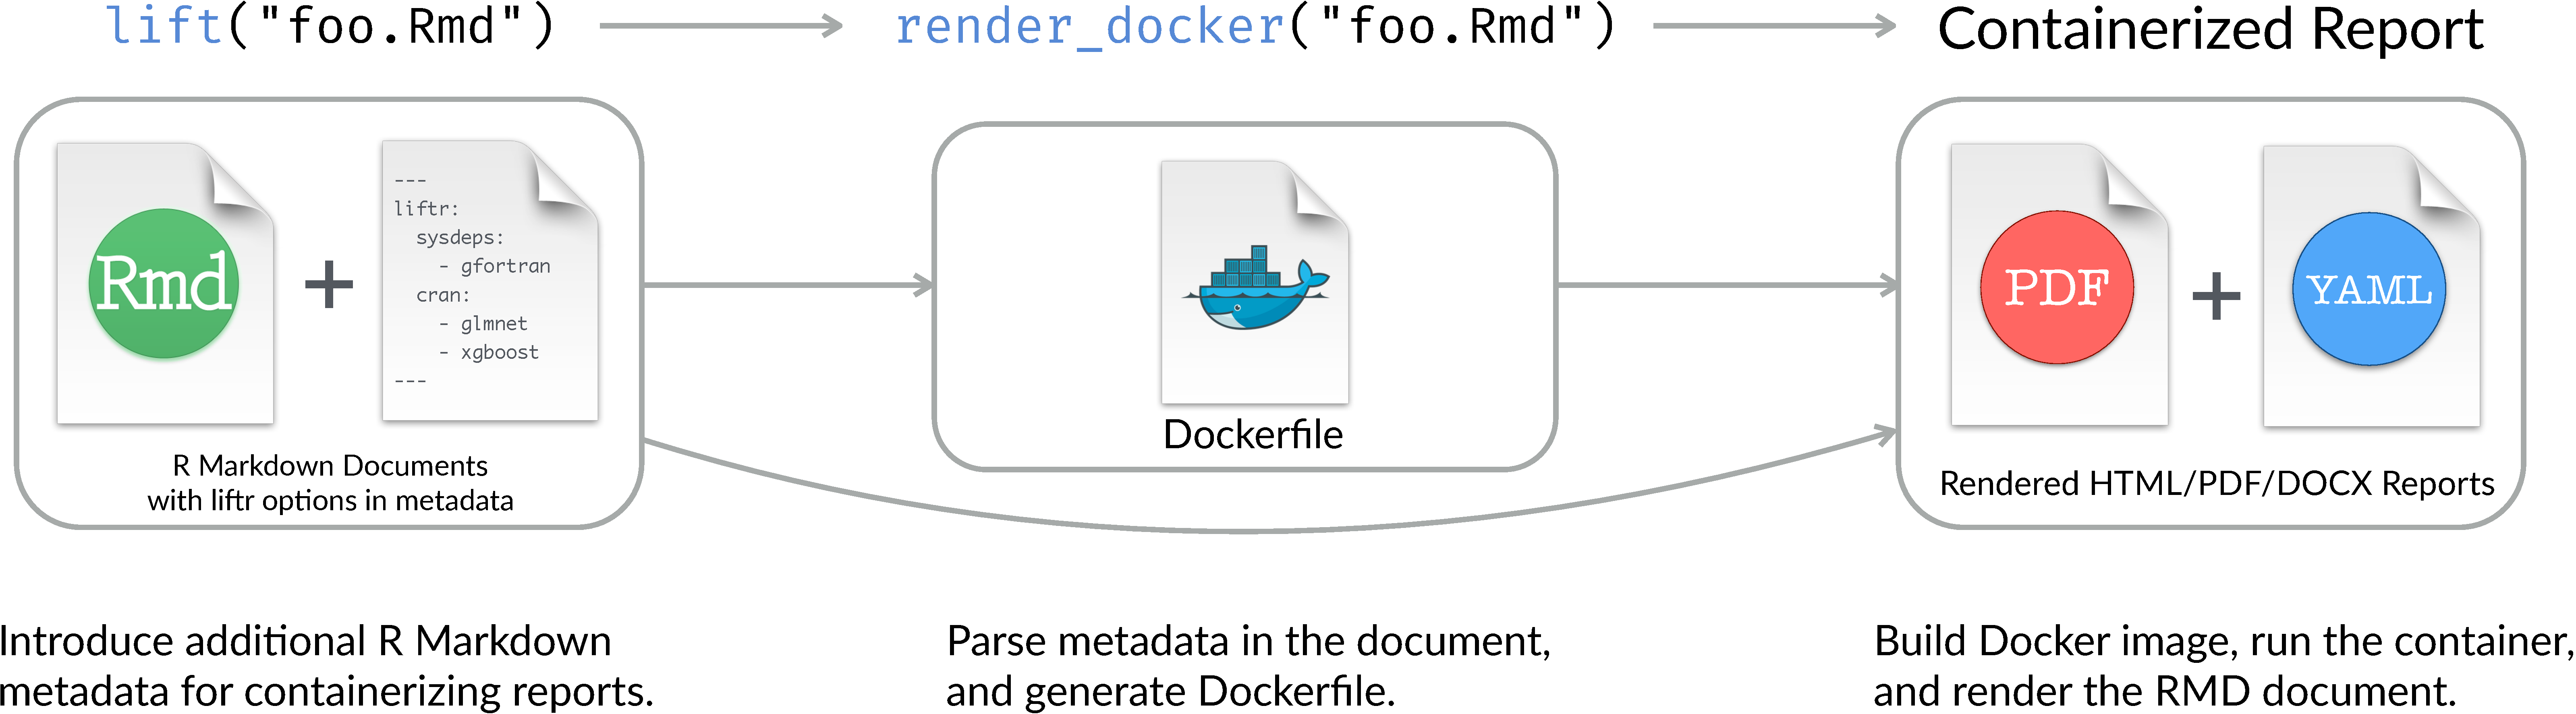
\includegraphics[width=\textwidth]{liftr-workflow}
  \caption{The liftr workflow for rendering containerized R Markdown documents.}
  \label{figure:liftr}
\end{figure}

\emph{knitr} and R Markdown are used as the template engine to generate
the \texttt{Dockerfile}. Features such as caching container layers for
saving image build time, automatic housekeeping for fault-tolerant
builds, and Docker status check are supported by \emph{liftr}. Four
RStudio addins are also offered by \emph{liftr} to allow push-button
compilation of documents and provide better IDE integrations.

Three basic principles are followed to design the \emph{liftr} package
since its inception.

\begin{enumerate}
\def\labelenumi{\arabic{enumi}.}
\item
  Continuous reproducibility. Continuous integration, continuous
  delivery, and continuous deployment are well-accepted practices in
  software engineering. Similarly, it is believed by the authors of
  \emph{liftr} that ensuring computational reproducibility means a
  continuous process instead of creating static data/code archives or a
  one-time deal. Specifically, the software packages used in data
  analysis should be upgraded regularly in a manageable way. Therefore,
  \emph{liftr} supports specifying particular versions of package
  dependencies, while users are encouraged to always use the latest
  version of packages (without a version number) by default.
\item
  Document first. Many data analysis workflows could be wrapped as
  either R packages or dynamic documents. In \emph{liftr}, the endpoint
  of dynamic report creation is the focus of containerization, because
  this offers more possibilities for organizing both computations and
  documentation. Users are encouraged to start thinking from the visible
  research output from the first day.
\item
  Minimal footprint. R Markdown and Docker are already complex software
  systems. Making them work together seamlessly can be complicated.
  Therefore, API designs such as function arguments are simplified while
  being kept as expressive and flexible as possible.
\end{enumerate}

In summary, \emph{liftr} tries to redefine the meaning of computational
reproducibility by offering system-level reproducibility for data
analysis. It provided a practical way for achieving it --- a new
perspective on how reproducible research could be done in reality.
Further, sharing system environments for data analysis also becomes
extremely easy, since users only need to share the R Markdown document
(with a few extra metadata fields), and compile them with \emph{liftr}.
As an example, \emph{liftr} demonstrated its advantage for R
Markdown-based computational workflow orchestration, by effortlessly
containerizing 18 complex \emph{Bioconductor} workflows in the DockFlow
project (\url{https://dockflow.org}) in 2017.

\begin{itemize}
\tightlist
\item
  \href{https://github.com/cole-brokamp/rize}{\texttt{rize} for Shiny}
\item
  \href{https://github.com/ColinFay/dockerfiler}{\texttt{dockerfiler}}
\end{itemize}

\hypertarget{packages-for-control-and-provisioning-richfitz-rcannoodnuest-richfitz-rcannood}{%
\subsection{\texorpdfstring{Packages for control and provisioning
{[}@nuest, @richfitz,
@rcannood{]}}{Packages for control and provisioning , @richfitz, @rcannood{[}@nuest, @richfitz, @rcannood{]}}}\label{packages-for-control-and-provisioning-richfitz-rcannoodnuest-richfitz-rcannood}}

\begin{itemize}
\tightlist
\item
  \href{https://github.com/richfitz/stevedore}{\texttt{stevedore}}
\item
  \href{https://cran.r-project.org/web/packages/babelwhale/index.html}{\texttt{babelwhale}}:
  Running a Docker from R with Singularity or Docker as back-end. This
  is really useful in HPC environments where a user might not have root
  access but is able to install Singularity instead of Docker.
  {[}@rcannood{]}
\item
  \href{https://bhaskarvk.github.io/docker/}{\texttt{docker}}
\item
  \texttt{RSelenium}
\item
  \href{https://cloudyr.github.io/googleComputeEngineR/}{\texttt{googleComputeEngineR}}
  (function \texttt{docker\_run})

  \begin{itemize}
  \tightlist
  \item
    I don't think \texttt{docker\_run} is main focus for containers for
    this package, its more how it uses Docker to launch custom
    environments that can be templated (e.g.~rstudio, shiny etc.) and
    for parrallisation e.g. \texttt{library(future)} using GCE VMs as
    endpoints. {[}@MarkEdmondson1234{]}
  \end{itemize}
\item
  \href{https://github.com/sckott/analogsea}{\texttt{analogsea}}
\item
  \href{https://github.com/wch/harbor/}{\texttt{harbor}}
\item
  \href{https://github.com/cboettig/dockermachine}{\texttt{dockermachine}}
\end{itemize}

\hypertarget{use-cases-and-applications}{%
\section{Use cases and applications}\label{use-cases-and-applications}}

\hypertarget{continuous-integration-and-continuous-delivery-colinfaynoamross-colinfay}{%
\subsection{\texorpdfstring{Continuous integration and continuous
delivery {[}@noamross,
@ColinFay{]}}{Continuous integration and continuous delivery , @ColinFay{[}@noamross, @ColinFay{]}}}\label{continuous-integration-and-continuous-delivery-colinfaynoamross-colinfay}}

\begin{itemize}
\tightlist
\item
  R-Hub
\item
  DevOps

  \begin{itemize}
  \tightlist
  \item
    \url{https://www.opencpu.org/posts/opencpu-with-docker/}
  \end{itemize}
\item
  \texttt{r-ci}: \url{https://github.com/ColinFay/r-ci}
\item
  \href{https://github.com/dynverse/dynwrap_containers/blob/master/.travis.yml}{dynwrap}
  {[}@rcannood{]}

  \begin{itemize}
  \tightlist
  \item
    For this project, we use travis-ci to build rocker-derived
    containers, test them, and only push them to docker hub (from
    travis-ci.org) if the integration tests succeed.
  \end{itemize}
\item
  Google Cloud Build {[}@MarkEdmondson1234{]}

  \begin{itemize}
  \tightlist
  \item
    \url{https://cloud.google.com/cloud-build/}
  \item
    For me this is what makes Docker containers viable, as it builds the
    Dockerfiles on each GitHub commit. It couples with Google Container
    Registry to build private Docker images, for downstream
    applications.
  \end{itemize}
\end{itemize}

\hypertarget{common-or-public-work-environments-div}{%
\subsection{Common or public work environments
{[}div{]}}\label{common-or-public-work-environments-div}}

\begin{itemize}
\tightlist
\item
  Binder

  \begin{itemize}
  \tightlist
  \item
    \href{https://github.com/karthik/holepunch}{\texttt{holepunch}}
    streamlines making an R research compendium Binder-ready
    {[}@karthik{]}
  \item
    \href{https://repo2docker.readthedocs.io/en/latest/config_files.html}{\texttt{repo2docker}}
    (\texttt{install.R}, \texttt{DESCRPTION}, \texttt{runtime.txt})
    based on the Rocker images {[}@nuest{]}
  \end{itemize}
\item
  GPU {[}@noamross, @cboettig{]}
\item
  Gigantum stack
\item
  in education (ready to use teaching/learning environments)

  \begin{itemize}
  \tightlist
  \item
    \href{https://github.com/ColinFay/r-db}{\texttt{r-db}}
    {[}@ColinFay{]}
  \end{itemize}
\item
  \href{https://github.com/att/rcloud/tree/master/docker}{RCloud} ?
\end{itemize}

\hypertarget{deployment-processing-cloud-div}{%
\subsection{Deployment, processing, cloud
{[}div{]}}\label{deployment-processing-cloud-div}}

\begin{itemize}
\tightlist
\item
  Docker images for cloud services {[}@MarkEdmondson1234{]}

  \begin{itemize}
  \tightlist
  \item
    the most popular functionality for \texttt{googleComputeEngineR} is
    its use of Docker to enable parallel processing across VMS -
    \href{https://cloudyr.github.io/googleComputeEngineR/articles/massive-parallel.html}{some
    demos here}
  \end{itemize}
\item
  Google Cloud Run - CaaS (Containers as a Service) that lets you launch
  a Docker container without worrying about underlying infrastructure.
  An R implementation is shown here at
  \href{https://github.com/MarkEdmondson1234/cloudRunR}{cloudRunR} which
  uses it to create a scalable R plumber API.
\item
  \href{https://www.rplumber.io/docs/hosting.html\#docker}{\texttt{plumber}}
\item
  \texttt{batchtools} \citep{Lang2017batchtools} can
  \href{https://mllg.github.io/batchtools/reference/makeClusterFunctionsDocker.html}{schedule
  jobs with Docker Swarm}
\item
  scalable deployments, e.g.~start with numerous Shiny talks mentioning
  Rocker at useR!2017
\item
  \href{https://github.com/dynverse/dynmethods}{dynmethods}
  {[}@rcannood{]}: In order to evaluate ±50 computational methods which
  all used different environments (R, Python, C++, \ldots{}), we wrapped
  each of them in a docker container and can execute these methods from
  R. Again, all of these containers are being built on travis-ci, and
  will only be pushed to docker hub if the integration test succeeds.
\item
  \href{https://www.shinyproxy.io/}{ShinyProxy}
  \href{https://github.com/openanalytics/shinyproxy/blob/master/src/main/java/eu/openanalytics/services/DockerService.java\#L388}{creates
  a container} for each user
\end{itemize}

\hypertarget{research-compendia-benmarwick}{%
\subsection{Research Compendia
{[}@benmarwick{]}}\label{research-compendia-benmarwick}}

\ldots{}

\hypertarget{other-containerisation-platforms-nn}{%
\section{Other containerisation platforms
{[}NN{]}}\label{other-containerisation-platforms-nn}}

\begin{itemize}
\tightlist
\item
  R images for Singularity
\item
  Running Rocker images with

  \begin{itemize}
  \tightlist
  \item
    Singularity
  \item
    CoreOS rkt?
  \end{itemize}
\item
  nix?
\end{itemize}

\hypertarget{discussionoutlookconclusion-please-add-bullet-pointsall-please-add-bullet-points}{%
\section{\texorpdfstring{Discussion/outlook/conclusion {[}@all, please
add bullet
points{]}}{Discussion/outlook/conclusion , please add bullet points{[}@all, please add bullet points{]}}}\label{discussionoutlookconclusion-please-add-bullet-pointsall-please-add-bullet-points}}

\begin{itemize}
\tightlist
\item
  Missing pieces?
\item
  consolidation (e.g.~via packages using \texttt{dockerfiler} and
  \texttt{stevedore})
\item
  Common themes

  \begin{itemize}
  \tightlist
  \item
    reproducibility
  \end{itemize}
\item
  will knowledge about containers continue to spread?
\item
  what is needed for even more containers with R?
\item
  the ability to move processing between services easily (e.g locally,
  one cloud providers VM, another cloud provider's
  Container-as-a-Service)
\item
  \ldots{}
\end{itemize}

\hypertarget{author-contributions}{%
\section{Author contributions}\label{author-contributions}}

DN conceived of the presented idea and
\href{https://github.com/nuest/rockerverse-paper/issues/3}{initialised the formation of the writing team}.
CB .. RC .. DE .. ME .. CF .. BW .. KR .. NR .. NX wrote the section on
liftr. LS \& NT wrote the section on Bioconductor. All authors
contributed to the discussion and outlook section and approved the final
version. This articles was collaboratively written at
\href{https://github.com/nuest/rockerverse-paper/}{https://github.com/nuest/rockerverse-paper/}.
The
\href{https://github.com/nuest/rockerverse-paper/graphs/contributors}{contributors page}
and
\href{https://github.com/nuest/rockerverse-paper/commits/master}{commit history}
provide a detailed view on the respective contributions.

\bibliography{RJreferences}


\address{%
Daniel Nüst\\
Institute for Geoinformatics, University of Münster\\
Heisenbergstr. 2, 48149 Münster, Germany\\
}
\href{mailto:daniel.nuest@uni-muenster.de}{\nolinkurl{daniel.nuest@uni-muenster.de}}

\address{%
Carl Boettiger\\
\\
\\
}


\address{%
Robrecht Cannoodt\\
\\
\\
}


\address{%
Dirk Eddelbuettel\\
University of Illinois at Urbana-Champaign\\
Department of Statistics\\ Illini Hall, 725 S Wright St\\ Champaign, IL 61820\\ ORCiD \href{https://orcid.org/0000-0001-6419-907X}{0000-0001-6419-907X}\\
}
\href{mailto:dirkd@eddelbuettel.com}{\nolinkurl{dirkd@eddelbuettel.com}}

\address{%
Mark Edmondson\\
IIH Nordic A/S, Google Developer Expert for GCP\\
\\
}
\href{mailto:mark@markedmondson.me}{\nolinkurl{mark@markedmondson.me}}

\address{%
Colin Fay\\
ThinkR\\
\\
}
\href{mailto:contact@colinfay.me}{\nolinkurl{contact@colinfay.me}}

\address{%
Ben Marwick\\
\\
\\
}


\address{%
Karthik Ram\\
\\
\\
}


\address{%
Noam Ross\\
\\
\\
}


\address{%
Nan Xiao\\
Seven Bridges Genomics\\
529 Main St, Suite 6610 \newline Charlestown, MA 02129, USA
\newline ORCiD: 0000-0002-0250-5673\\
}
\href{mailto:me@nanx.me}{\nolinkurl{me@nanx.me}}

\address{%
Lori Shepherd\\
Roswell Park Comprehensive Cancer Center\\
Elm \& Carlton Streets, Buffalo, New York, 14263 USA\\
}
\href{mailto:lori.shepherd@roswellpark.org}{\nolinkurl{lori.shepherd@roswellpark.org}}

\address{%
Nitesh Turaga\\
Roswell Park Comprehensive Cancer Center\\
Elm \& Carlton Streets, Buffalo, New York, 14263 USA\\
}
\href{mailto:nitesh.turaga@roswellpark.org}{\nolinkurl{nitesh.turaga@roswellpark.org}}

